\chapterstart{BabyLM 2026：有限经验学习的研究前沿}
\label{sec:intro}

当语言模型已经能够利用海量文本学习时，为什么还要研究只读过少量文本的模型？这个问题涉及人工智能发展的另一条重要路径：除了扩大训练规模，能否让每一份经验产生更多知识，让已经学到的知识适用于新的表达，并在继续学习时保留下来？训练出一个规模更大的模型，回答了能力可以随资源增长到什么程度；在严格的数据约束下训练出更好的模型，则有助于辨明学习方法本身还有多少改进空间。

BabyLM 为后一类研究建立了公开的共同实验条件。本报告研究其中的 Strict-Small 赛道，并呈现 Qiushi Engine 如何从前沿模型的创造出发，研究有效方法背后的条件，再据此改进模型。两代模型的成绩是这项研究的可见结果；从实验中形成、能够被继续检验和使用的认识，是另一项同样重要的产出。

\subsection{有限经验学习的科学问题}

语言模型通过预测文本学习。训练先比较模型对候选词的预测概率与文本中实际出现的词，再用一个称为损失的数值衡量预测偏差，据此调整模型参数。本文所说的监督，就是指定哪些预测参与这种学习；监督目标是要求模型恢复的词，监督位置是这些词在输入中的位置。经过反复学习，模型逐渐掌握词语搭配、句法、语义及上下文中的联系。研究还需要辨明：正确预测究竟来自所需的信息关系，还是来自容易利用的局部线索。

例如，前文说明“钥匙从抽屉移到了盒子”，后文询问钥匙现在的位置。模型需要利用前文的状态变化，而不能只依靠“钥匙”和“抽屉”经常一起出现的经验。如果训练中附近词语已经足以猜出答案，模型可以降低预测错误，却很少练习追踪前文。这里的关键区别是：\textbf{接触过相关信息，与学会在需要时使用这些信息，是两回事。}

有限数据条件使这一区别更加突出。新增一段文本、重复一段旧文本、把同一内容改写成另一种表达，都会占用训练预算，却未必提供相同的学习机会。重复可以巩固已有模式；不同表达可能帮助模型跨越词面变化；新增来源可以扩展内容覆盖。怎样分配这些机会，需要同时考虑模型已经学会什么、还缺少什么，以及剩余预算允许进行多少学习。数据受限的标度研究也表明，重复使用已有数据的价值需要与不重复的原始数据量及训练配置一起分析\citep{muennighoff2025scaling}。

“数据高效语言建模”研究怎样更充分地利用有限的学习材料。模型参数量、训练语料量、累计文本呈现量与计算成本分别描述模型容量、材料规模、接触经验的次数与执行代价。小模型也可能反复读过大量文本，较大的模型也可能只有有限经验。BabyLM 的英语严格赛道同时限制语料池规模与累计文本呈现量，让研究者在共同的数据约束下比较数据组织、模型结构和学习方法。

本研究将问题进一步聚焦为：\textbf{什么样的训练经验能够让模型学会利用上下文中的信息关系，并使这种能力在后续学习中仍然可用？}本文将完成预测需要利用的上下文信息及其关系称为\textbf{上下文依赖}。这一问题连接了语言学习、组合泛化和持续学习：组合泛化指把学过的成分用于新的组合，持续学习则研究怎样在学习新能力时保留原有能力。后文分别用自然文本、受控关系任务和真实模型训练检验这些问题。

\subsection{研究背景与赛道设置}
\label{sec:setting}

BabyLM 始于 2023 年，2026 年进入第四届，作为共享任务和专题研讨会与 EMNLP 2026 关联。它连接自然语言处理、计算认知科学与语言习得研究，提供训练数据、评价程序、基线模型和公开比较平台\citep{warstadt2023babylm,babylm2026website}。历届任务总结与论文进一步积累了数据处理、模型构造和学习行为方面的研究\citep{charpentier2025babylm}。

这一设置的学术价值来自问题和实验条件，而不只来自榜单。对机器学习研究者，它提供可重复比较训练方法的环境；对语言与认知研究者，它提供观察知识怎样随经验形成的计算模型；对资源有限的研究团队，它使从头预训练、保存中间模型和开展对照实验更容易实施。它并不要求机器完整模拟儿童，而是把受限输入下的语言学习作为机器学习与认知研究可以共同讨论的对象。

2026 年的赛道包括英语 Strict-Small、英语 Strict，以及面向英语、荷兰语和中文的 Multilingual。本报告只研究 Strict-Small，不混合不同赛道的成绩。与本研究直接相关的两级英语预算如下\citep{choshen2026babylm}。

\begin{table}[htbp]
\caption{英语赛道的两个数据约束。M 表示百万；单词数按赛道规则统计，不是模型分词后的 token 数。}
\label{tab:tracks}
\begin{tabularx}{\linewidth}{@{}P{45mm}YY@{}}
\toprule 赛道 & 训练语料池上限 & 累计训练曝光上限\\\midrule
Strict-Small（本研究） & 10M 词，即一千万词 & 100M 词，即一亿词\\
Strict & 100M 词，即一亿词 & 1B 词，即十亿词\\
\bottomrule
\end{tabularx}
\end{table}

语料池是可以用于训练的文本集合，累计曝光是模型训练过程中实际接触文本的总量。两者不能混为一谈：同一篇一千词的文章读十遍，仍是一篇文章，却已经消耗一万词的曝光预算。改写文本、重复呈现和为保持旧能力而再次输入的文本，也需要按适用规则记账。模型将单词切分为更小的计算单元，这些单元称为 token；一个单词可以对应多个 token，因此模型的分词计数不能直接替代赛道的单词计数。

官方还要求保存中间检查点，即不同训练进度的模型权重，以评价学习过程。外部教师生成文本及其他辅助训练方式有单独的规则，不能仅凭最终词数确认全部条件；本研究的数据和教师说明见附录\ref{app:repro}。这些要求使比较不仅关心最终得分，也关心模型通过什么经验和训练过程达到该结果。

预算固定之后，研究空间仍然开放。研究者需要选择数据内容与表达形式、词表、模型结构、预测目标、学习率、批量大小、训练顺序和模型选择方法。其中，学习率决定一次更新改变参数的幅度，批量大小决定一次更新汇总多少训练样本；两者都不是越大或越小越好。相同词预算下，更大的批量还可能意味着更少的更新次数。Strict-Small 因而不是一份已经给出全部训练答案的配方，而是一组允许检验不同答案的共同约束。

\subsection{语言能力与学习行为的评价体系}

一个语言模型能否学会语法、追踪变化中的对象、利用常识、把已有表示用于新任务，以及呈现接近人类的语言行为，需要不同的测量。BabyLM 的九项一级指标分别观察这些能力和行为。\textbf{评价体系同时包含语言任务表现与人类行为对应程度，总分汇总的是不同类型的测量。}理解分数时，应先区分每项指标的任务、计算方式和参照水平。

\begin{table}[htbp]
\caption{BabyLM 英语评价的九个一级指标。前七项构成 NLP Average，后两项构成 Human-like Average。具体数值按固定版本的官方兼容实现计算。}
\label{tab:metrics}
\small
\begin{tabularx}{\linewidth}{@{}P{31mm}Y Y@{}}
\toprule 指标 & 主要检验什么 & 怎样理解分数\\\midrule
BLiMP & 能否区分只有细微差别的合语法与不合语法句子 & 多类语法现象上的选择准确率。\\
BLiMP Supplement & 问答、指称等补充语言现象 & 多组补充任务单独汇总。\\
EWoK & 能否根据情境调用基本世界知识 & 比较后续表达在不同情境中的合理性。\\
Entity Tracking & 对象经过移动或更新后，能否找到其当前状态 & 状态操作后的候选答案准确率。\\
COMPS & 能否把属性用于新概念，并抵抗无关信息干扰 & 概念属性、继承和干扰条件的比较。\\
GlobalPIQA & 能否判断日常物理行为和用途 & 不同题型子集的选择准确率。\\
(Super)GLUE & 预训练表示能否支持后续语言理解任务 & 规定微调后的任务指标均值。\\
Reading & 模型预测能否解释人类阅读行为中的变化 & 控制词频、词长等因素后的解释增益。\\
AoA & 模型学习词汇的先后是否与儿童习得顺序相关 & 多个训练检查点上的轨迹相关指标。\\
\bottomrule
\end{tabularx}
\end{table}

\subsubsection{语言形式、知识与上下文使用}

BLiMP 的最小句对将细微的语法区别单独提取出来，例如主谓一致；EWoK 改变情境，检查模型是否随之改变对表达的判断；COMPS 检查新概念能否继承合适的属性，以及无关概念是否会干扰判断；Entity Tracking 则要求在一连串操作后仍能找到正确状态\citep{warstadt2020blimp,ivanova2025ewok,misra2023comps,kim2023entity}。这些任务使“句子看起来流畅”与“确实利用了所需信息”能够被分别评价。

例如，句子“The keys are on the table”涉及主谓一致；“钥匙先放进抽屉，随后移入盒子”涉及状态更新；给一种新命名的动物指定类别，再判断它应具有什么属性，涉及概念继承。这里的例子用于解释能力区别，并非实际测试题。它们也说明，小模型的研究困难并不只是背诵事实：有限经验需要支持结构规则、关系使用与状态变化等不同计算。

这些评测通常直接使用预训练模型比较句子或候选答案的得分，不先针对每道题训练模型，称为零样本评测。机会水平取决于题型，不能统一当成 50\%。例如，本报告的 GlobalPIQA 英语评测包含 103 道四选一题和 100 道二选一题；两子集等权汇总，均匀随机选择的期望为 37.5 分。因而，同样是 40 分，若题型、机会水平或评分方法不同，所反映的能力也不同\citep{chang2026globalpiqa,babylm2026evaluation}。

\subsubsection{后续任务中的表示迁移}

(Super)GLUE 测量的是另一种能力：模型经过规定的任务训练后，是否能够支持语言理解。这种在预训练基础上的任务训练称为微调。BabyLM 使用七个任务的选集，包括是非问答、文本蕴含、句子或问题是否同义、多句阅读判断与指代消解\citep{wang2018glue,wang2019superglue}。它检验预训练所得表示能否成为新任务的有效基础。

这些任务有的采用准确率，有的采用 F1。准确率统计答对比例；F1 同时考虑某一类答案预测得是否准确、是否找得完整。因此，(Super)GLUE 不是原版基准的全部任务，也不是全部题目混在一起的正确率。微调随机性、分类头、训练设置和模型选择均可能影响结果，需要在比较中保持一致。

\subsubsection{阅读行为与词汇习得}

Reading 不考查模型阅读一篇文章后答对多少问题，而是研究模型对词语的预期与人类阅读行为之间的联系。给定前文，一个词出现的概率越低，它对模型越“意外”。这个意外程度用负对数概率表示，英文为 surprisal。评价检验它能否在词长、词频等因素之外，进一步解释眼动或逐词阅读时间的变化\citep{devarda2024cloze}。

本文采用 BabyLM 2026 评测程序的评分定义\citep{babylm2026evaluation}。若仅使用控制变量时解释的变异比例为 $R_0^2$，加入模型预测后为 $R_1^2$，相应的归一化增益为
\begin{equation}
 q=\frac{R_1^2-R_0^2}{1-R_0^2}.
\end{equation}
例如，从解释 20\% 增至 24\%，增益为 $0.04/0.80=0.05$，按百分制表达为 5 分。这个公式例子说明了为什么较小的 Reading 数值仍有实际测量含义：它衡量控制变量之外的增量解释量，而非阅读准确率。榜单再按规定汇总不同阅读响应\citep{babylm2026leaderboard}。

AoA 是 Age of Acquisition，即词汇习得年龄。评价利用多个中间模型上同一词的预测曲线，估计其学习进度，再与儿童词汇习得顺序比较\citep{chang2022word}。本文采用的评测实现计算 Pearson 相关；有效词少于三个或相关检验的 $p>0.1$ 时记为零，通过门限的负相关则保留负分\citep{babylm2026evaluation}。具体评分版本与检查点轨迹见附录\ref{app:evaluation}。\textbf{AoA 为零并不表示模型一个词也没有学会。}它与 Reading 一起，使语言任务能力和人类行为对应程度能够被分别研究。

\subsection{综合评价与排行榜解释}

令九个一级分数为 $m_1,\ldots,m_9$，七项语言任务的均值为 $N$，两项人类行为指标的均值为 $H$。Overall Average 的计算为
\begin{equation}
 O=\frac{1}{9}\sum_{j=1}^{9}m_j=\frac{7N+2H}{9}.
\label{eq:overall}
\end{equation}
九项分别等权，所以 NLP 与 Human-like 的总权重并不相等。Overall 汇总了不同能力与行为指标，适合按同一协议比较模型；它不能读成“模型只会 42\% 的语言”，也不能与大型模型在其他试题、其他训练预算上的得分直接比较。

本研究的两代代表模型分别为 \nolinkurl{Qiushi-Engine-Frontier-Advancement} 和 \nolinkurl{Qiushi-Engine-Principle-Guided-Frontier-Advancement}，下文简称 \Frontier{} 与 \Guided{}。第一代公开 Overall 为 42.02，第二代提高至 42.25，在本报告保存的公开 Strict-Small 快照中达到最高 Overall。它们展示了从前沿模型到原理指导改进的实际进展。

表\ref{tab:board}只列两代正式模型，并补入其他发布者中 Overall 最高的八项。这里比较的是公开方法，不列本团队历史提交，也不显示或重新编排排名。快照为 2026 年 9 月 8 日 20:53（北京时间）的公开记录；比较以 Overall 为准，公开榜单与当届比赛奖项的认定是不同事项\citep{babylm2026leaderboard}。

\begin{table}[htbp]
\caption{两代代表模型与八项外部公开提交的比较。模型使用可读简称，完整名称与链接随数据表提供；分数保留公开显示精度。}
\label{tab:board}
\small
\begin{tabularx}{\linewidth}{@{}Yrrr@{}}
\toprule 发布者／模型 & Overall & NLP & Human-like\\\midrule
\input{tables/leaderboard}
\end{tabularx}
\end{table}

\begin{figure}[htbp]
\centering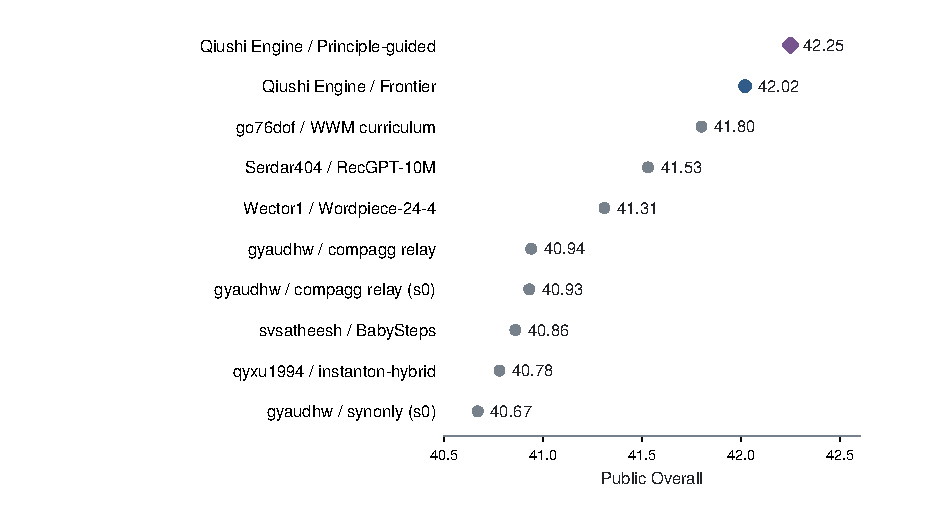
\includegraphics[width=\linewidth]{figures/leaderboard.pdf}
\caption{BabyLM 2026 Strict-Small 公开模型的 Overall 比较（2026 年 9 月 8 日）。展示两代 Qiushi Engine 模型与八项外部提交，点及其标签表示公开分数；比较对象与表\ref{tab:board}一致。}
\label{fig:leaderboard}
\end{figure}

八项外部提交集中在 40.67 至 41.80，跨度为 1.13 分，相邻条目的差距可低至 0.01。第二代相对外部最高显示分数提高 0.45。接近的总分使方法比较需要更细致的分项分析：哪些能力提高了，哪些发生了取舍，以及同一起点上的重复训练是否仍有收益。公开分数展示前沿位置，后文的共同母模型对照进一步检验训练方案的贡献。

总分相近还可能隐藏不同的能力结构。比较组中，最高 NLP 为 53.59，却因人类行为指标较弱而未取得最高 Overall。BLiMP 为 67.13--73.11，Entity Tracking 为 16.59--29.40；GlobalPIQA 为 36.08--40.68，接近其 37.5 的随机参照。这些差异表明，句法偏好、动态状态与物理常识尚未同步解决。附录\ref{app:board}保留全部九项分数，避免让一个总分掩盖各方法的长处与代价。

\subsection{有限经验学习的关键挑战}

\textbf{经验覆盖与重复练习之间的取舍。}有限的词预算既可以用于更多内容，也可以用于反复巩固已有内容。把文本压缩得更短，可能让更多材料进入预算，也可能丢掉关系线索；改写可能增加表达变化，也可能只制造冗余。研究需要检验哪些处理真正改变了学习，而不能仅按文本数量或流畅程度判断质量。

\textbf{正确预测与有效信息利用之间的区别。}模型可能通过目标附近的搭配完成预测，没有使用相关来源。训练损失下降是真实的，却未必意味着所需关系能力已经形成。为辨明这一点，需要保持预测目标不变，改变可见线索；或保持文本不变，改变哪些词承担学习目标。后文的输入遮盖与监督位置实验正是围绕这两个变量展开。

\textbf{新能力学习与旧能力保持之间的协调。}针对某一种关系训练，可能使模型更会处理这一类题，却损伤普通语言任务。即便熟悉题目的表现恢复，新名字、新表达仍可能无法使用原来的计算。综合改善要求把新能力和已有功能同时测量，不能只在最容易上涨的一个指标上宣布成功。

\textbf{结构、优化与训练过程之间的相互作用。}分词决定文本怎样进入模型；结构决定它能表达什么；学习目标和优化决定哪些关系得到反复训练。一个在早期较好的方案可能在后期失去优势，同样的随机种子也未必使不同结构拥有相同初值。严格比较需要识别这些差别，并选择真正能区分解释的实验。

\textbf{模型训练与科学研究的成本不同。}一次模型训练在预算内，不代表找到该方法的整个过程只花费同样资源。方案筛选、机制对照、完整评测和误差分析都需要工作。对自主研究系统而言，困难在于连续完成这些环节：保留可靠起点，识别有价值的问题，安排对照，发现错误，修正解释，再将认识转化为可以运行的新方法。Qiushi Engine 的研究能力应从这一连续过程理解，而非仅从最后一次训练理解。

\subsection{性能增量与科学贡献}

前沿模型的改进需要同时考虑分数、比较条件和科学解释。由于 Overall 是九项均值，某一分项上升 0.9 分、其余不变，会使 Overall 上升 0.1 分；多项小幅变化也可以累积出同样结果。因此，一个小的总分差值可能来自真实而明确的行为变化，也可能受到样本规模、训练随机性或模型选择影响。必须回到分项和对照，才能判断它说明了什么。

本研究不仅比较第一代与第二代，还设置从同一第一代模型出发的普通续训：如果新方案只是多训练一段，它应当难以持续超过这个参照。在两个续训随机种子下，普通续训的完整 Overall 为 42.0926 和 42.1159；密集遮盖、稀疏监督方案在相同累计词曝光下达到 42.2025 和 42.1789。加入普通输入保持的完整方案进一步达到 42.2464 和 42.2317。保持方案增加了部分输入呈现，后文分别说明整体效果与因素归因。

这些成绩的意义不止于位次变化。第一阶段留下了压缩表达并重新分配经验预算的方法、可以继续学习的模型结构，以及完整训练与评测基础。第二阶段进一步发现，不同的重复和重述关系会塑造不同的上下文使用行为，熟悉表现与新输入上的复用也可以分离。第三阶段把这些认识落实为训练操作，并由实际模型结果检验。\textbf{科学贡献由新的现象、可区分的解释、可操作的方法及其证据共同构成，不能由榜单差值单独替代。}

研究还考察了少量标签怎样帮助确定关系、新名字怎样与已知对象建立对应，以及显式记忆怎样读取正确状态。这些问题分别形成关系锚点、身份匹配与实体记忆等独立研究方向。它们扩展了对有限经验学习的认识，第\ref{sec:lineage}章将分别说明其构造、发现和适用条件。

\subsection{研究价值与应用前景}

有限数据研究的直接产出是能够被比较和重用的学习方法。专业领域、低资源语言及数据获取受限的应用，常面临高质量训练材料不足的问题。如何保留关键信息、组织互相对应的表达、安排监督与继续学习，因而具有潜在的迁移价值。本研究提供了相应的方法与实验依据，向这些应用迁移是后续可具体检验的方向。

对大规模预训练而言，小规模研究提供了更容易实施的机制实验条件。研究者可以控制数据和训练变量，检查一种方法为什么有效。局部预测捷径、监督分配失衡和保持约束过强等发现，为更大规模训练提供了明确的待检验假设。后续比较可进一步考察这些条件如何随模型规模、任务与预算变化。

对语言与认知科学而言，模型提供了可以操纵输入经验、追踪学习变化的实验对象。语法判断、概念继承、阅读行为和习得轨迹的联合评价，允许研究者讨论“任务表现更好”与“学习过程更接近人类”何时一致、何时分离。模型不是人类学习的完整替身，但清楚的对照可以使两类研究形成实质联系。

对自主人工智能研究而言，本项目将前沿探索、科学认识和方法创造纳入同一个长期研究过程。Qiushi Engine 持续发展数据构造、模型设计与实验方法，也根据新证据调整问题和路线。我们以 Research RSI——科研过程的递归自我改进——描述这种积累重新进入后续研究的过程。第\ref{sec:rsi}节说明其具体实现、与相关工作的联系及实证范围。

\subsection{Qiushi Engine 的三阶段自主研究}

Qiushi Engine 主导并执行了贯穿三个阶段的科学研究，包括文献研究、问题与假设形成、数据构造、模型及学习目标设计、实验实现、评测分析和成果整合。团队提供研究目标、资源和阶段性要求，系统在这些条件下持续开展自主研究。计算工作基于 AI Lab 技能与配套科研程序，覆盖数据生成、模型训练、评测和机制实验，由两张 NVIDIA H100 GPU 与 CPU 支持。研究组织见第\ref{sec:research_organization}节，计算环境见附录\ref{app:compute}。

三个阶段围绕同一个科学问题展开，每个阶段都是包含问题提出、假设与方法构造、实验执行、证据分析和成果整理的完整研究过程。它们逐步扩展研究的深度：先在开放的设计空间中创造前沿模型，再从成功、失败与方法分歧中研究学习条件，最后将形成的原理与技术用于新的模型创造。模型、数据、算法和实验方法持续积累，科学解释则接受后续证据的检验与修正。

\textbf{第一阶段，前沿突破。}从有限数据下的模型训练出发，联合探索文本构造、分词与表示、模型结构、优化和训练安排。紧凑重述、预算再分配与残差增量学习逐渐形成可共同使用的方案，经过训练与完整评测产生第一代前沿模型。研究同时留下了数据构造、模型实现和实验基础，以及早晚期效果不同、局部学习与综合表现不一致等需要解释的现象。

\textbf{第二阶段，原理发现。}把第一阶段积累的模型与现象转化为研究对象，提出竞争解释，再通过数据、窗口、监督、表示和内部计算的干预逐步检验。研究涉及经验结构与压缩、表示与归纳偏置、学习信号与能力保持、课程与学习动力学，以及测量和计算实现。关系学习与能力复用形成连接下一阶段的主要认识；关系锚点、身份匹配、初始化对齐和测量方法等研究，也留下了各自独立的发现与工具。

\textbf{第三阶段，原理指导的模型改进。}从已有认识提出新的训练设计，在继承第一代模型和文本的条件下，分别改变预测时可见的信息、承担监督的位置和保持约束。普通续训、不同目标配置、机制检验与完整评测共同检验方案，产生第二代模型，也进一步修正关于监督数量和保持强度的解释。图\ref{fig:program}概括三个完整研究过程的连续积累。

\begin{figure}[H]
\centering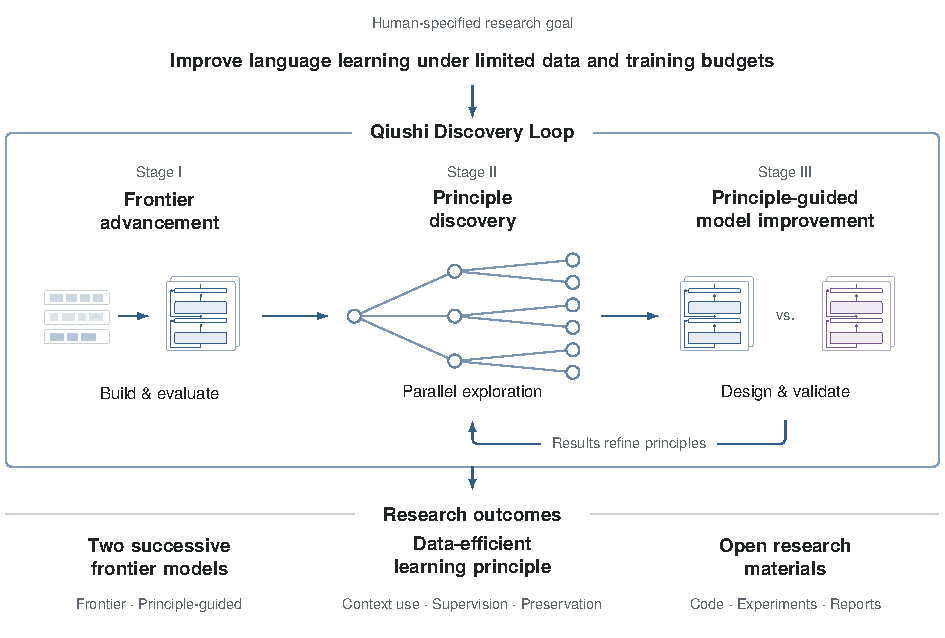
\includegraphics[width=\linewidth]{figures/three_stage_research_public.pdf}
\caption{Qiushi Engine 的三阶段自主研究。前沿探索、原理发现与原理指导的模型改进各自包含完整研究过程；模型、方法与科学认识在阶段之间积累和发展。研究形成两代前沿模型、数据高效学习原则与开放研究材料。}
\label{fig:program}
\end{figure}

这些研究支持一项可检验的数据高效学习设计原则（data-efficient learning principle）：\textbf{围绕目标能力所需的上下文依赖组织有限经验，使相关信息在预测时可用，让监督训练模型利用这些信息，并分别检验能力的获得、复用与保持。}获得指学会目标任务，复用指新对象或新表达能够使用所学能力，保持指后续学习后这些能力仍然可用。第\ref{sec:principles}、\ref{sec:guided}章分别说明原则的实验依据、训练设计与作用条件。
